


\tikzset{every picture/.style={line width=0.75pt}} %set default line width to 0.75pt        

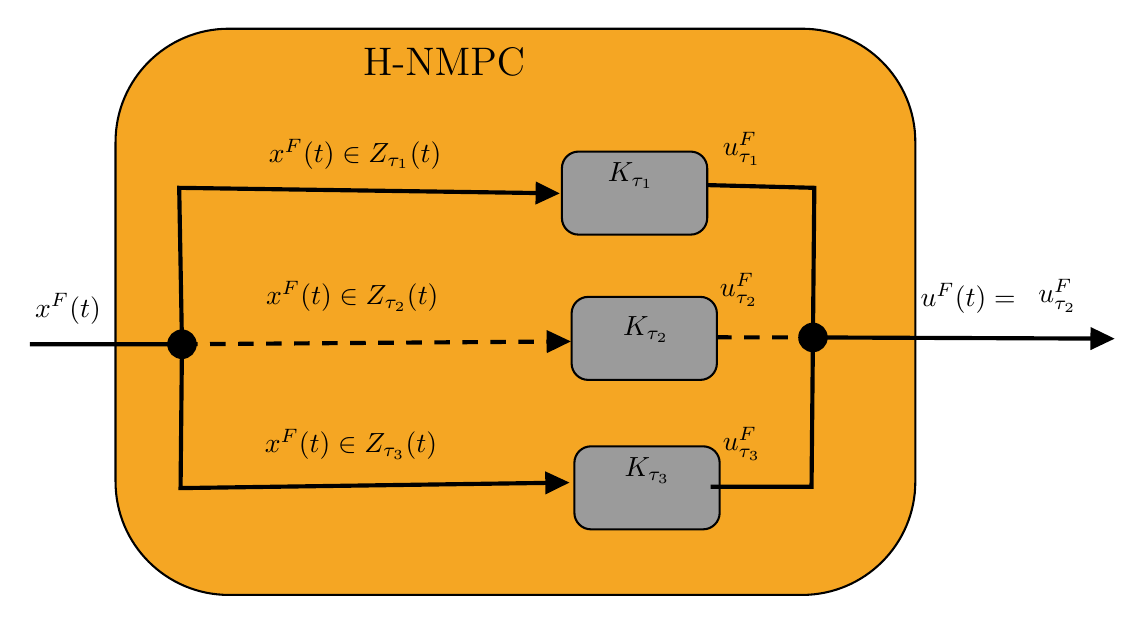
\begin{tikzpicture}[x=0.75pt,y=0.75pt,yscale=-1,xscale=1]
	%uncomment if require: \path (0,300); %set diagram left start at 0, and has height of 300
	
	%Rounded Rect [id:dp29292135946148945] 
	\draw  [fill={rgb, 255:red, 245; green, 166; blue, 35 }  ,fill opacity=1 ] (129.6,78.43) .. controls (129.6,48.29) and (154.03,23.87) .. (184.16,23.87) -- (460.37,23.87) .. controls (490.51,23.87) and (514.93,48.29) .. (514.93,78.43) -- (514.93,242.11) .. controls (514.93,272.24) and (490.51,296.67) .. (460.37,296.67) -- (184.16,296.67) .. controls (154.03,296.67) and (129.6,272.24) .. (129.6,242.11) -- cycle ;
	%Rounded Rect [id:dp5735225713311956] 
	\draw  [fill={rgb, 255:red, 155; green, 155; blue, 155 }  ,fill opacity=1 ] (344.67,91.07) .. controls (344.67,86.65) and (348.25,83.07) .. (352.67,83.07) -- (406.67,83.07) .. controls (411.08,83.07) and (414.67,86.65) .. (414.67,91.07) -- (414.67,115.07) .. controls (414.67,119.48) and (411.08,123.07) .. (406.67,123.07) -- (352.67,123.07) .. controls (348.25,123.07) and (344.67,119.48) .. (344.67,115.07) -- cycle ;
	%Rounded Rect [id:dp49775197703290064] 
	\draw  [fill={rgb, 255:red, 155; green, 155; blue, 155 }  ,fill opacity=1 ] (349.33,161.07) .. controls (349.33,156.65) and (352.92,153.07) .. (357.33,153.07) -- (411.33,153.07) .. controls (415.75,153.07) and (419.33,156.65) .. (419.33,161.07) -- (419.33,185.07) .. controls (419.33,189.48) and (415.75,193.07) .. (411.33,193.07) -- (357.33,193.07) .. controls (352.92,193.07) and (349.33,189.48) .. (349.33,185.07) -- cycle ;
	%Rounded Rect [id:dp7692690786653456] 
	\draw  [fill={rgb, 255:red, 155; green, 155; blue, 155 }  ,fill opacity=1 ] (350.67,233.07) .. controls (350.67,228.65) and (354.25,225.07) .. (358.67,225.07) -- (412.67,225.07) .. controls (417.08,225.07) and (420.67,228.65) .. (420.67,233.07) -- (420.67,257.07) .. controls (420.67,261.48) and (417.08,265.07) .. (412.67,265.07) -- (358.67,265.07) .. controls (354.25,265.07) and (350.67,261.48) .. (350.67,257.07) -- cycle ;
	%Straight Lines [id:da5301562617313751] 
	\draw [line width=1.5]  [dash pattern={on 5.63pt off 4.5pt}]  (161.61,175.89) -- (161.61,175.89) -- (344.93,174.56) ;
	\draw [shift={(348.93,174.53)}, rotate = 179.59] [fill={rgb, 255:red, 0; green, 0; blue, 0 }  ][line width=0.08]  [draw opacity=0] (11.61,-5.58) -- (0,0) -- (11.61,5.58) -- cycle    ;
	%Straight Lines [id:da6683179377534789] 
	\draw [line width=1.5]    (161.61,175.89) -- (160.93,245.2) -- (344.27,242.59) ;
	\draw [shift={(348.27,242.53)}, rotate = 179.18] [fill={rgb, 255:red, 0; green, 0; blue, 0 }  ][line width=0.08]  [draw opacity=0] (11.61,-5.58) -- (0,0) -- (11.61,5.58) -- cycle    ;
	%Straight Lines [id:da3146810547564285] 
	\draw [line width=1.5]    (161.61,175.89) -- (160.27,100.53) -- (339.6,103.14) ;
	\draw [shift={(343.6,103.2)}, rotate = 180.83] [fill={rgb, 255:red, 0; green, 0; blue, 0 }  ][line width=0.08]  [draw opacity=0] (11.61,-5.58) -- (0,0) -- (11.61,5.58) -- cycle    ;
	%Shape: Circle [id:dp11620000253813201] 
	\draw  [fill={rgb, 255:red, 0; green, 0; blue, 0 }  ,fill opacity=1 ] (155.01,175.89) .. controls (155.01,172.24) and (157.96,169.28) .. (161.61,169.28) .. controls (165.26,169.28) and (168.22,172.24) .. (168.22,175.89) .. controls (168.22,179.54) and (165.26,182.5) .. (161.61,182.5) .. controls (157.96,182.5) and (155.01,179.54) .. (155.01,175.89) -- cycle ;
	%Straight Lines [id:da25743336719109333] 
	\draw [line width=1.5]    (88.27,175.87) -- (161.61,175.89) ;
	%Shape: Circle [id:dp4553392259587261] 
	\draw  [fill={rgb, 255:red, 0; green, 0; blue, 0 }  ,fill opacity=1 ] (459.01,172.61) .. controls (459.01,168.96) and (461.96,166) .. (465.61,166) .. controls (469.26,166) and (472.22,168.96) .. (472.22,172.61) .. controls (472.22,176.26) and (469.26,179.22) .. (465.61,179.22) .. controls (461.96,179.22) and (459.01,176.26) .. (459.01,172.61) -- cycle ;
	%Straight Lines [id:da7934163199862663] 
	\draw [line width=1.5]  [dash pattern={on 5.63pt off 4.5pt}]  (418.95,172.55) -- (418.95,172.55) -- (465.61,172.61) ;
	%Straight Lines [id:da8204927248858007] 
	\draw [line width=1.5]    (414.95,99.22) -- (414.95,99.22) -- (466.27,100.53) -- (465.61,172.61) ;
	%Straight Lines [id:da6576991924158868] 
	\draw [line width=1.5]    (416.34,244.55) -- (416.34,244.55) -- (464.93,244.53) -- (465.61,172.61) ;
	%Straight Lines [id:da5383508392621161] 
	\draw [line width=1.5]    (465.61,172.61) -- (606.93,173.18) ;
	\draw [shift={(610.93,173.2)}, rotate = 180.23] [fill={rgb, 255:red, 0; green, 0; blue, 0 }  ][line width=0.08]  [draw opacity=0] (11.61,-5.58) -- (0,0) -- (11.61,5.58) -- cycle    ;
	
	% Text Node
	\draw (247.33,32) node [anchor=north west][inner sep=0.75pt]  [font=\Large] [align=left] {H-NMPC};
	% Text Node
	\draw (365.33,87.07) node [anchor=north west][inner sep=0.75pt]    {$K_{\tau _{1}}$};
	% Text Node
	\draw (372.67,161.07) node [anchor=north west][inner sep=0.75pt]    {$K_{\tau _{2}}$};
	% Text Node
	\draw (373.33,229.07) node [anchor=north west][inner sep=0.75pt]    {$K_{\tau _{3}}$};
	% Text Node
	\draw (89.33,150.07) node [anchor=north west][inner sep=0.75pt]    {$x^{F}( t)$};
	% Text Node
	\draw (202,75.4) node [anchor=north west][inner sep=0.75pt]    {$x^{F}( t) \in Z_{\tau _{1}}( t) \ $};
	% Text Node
	\draw (200.67,144.07) node [anchor=north west][inner sep=0.75pt]    {$x^{F}( t) \in Z_{\tau _{2}}( t) \ $};
	% Text Node
	\draw (200,215.4) node [anchor=north west][inner sep=0.75pt]    {$x^{F}( t) \in Z_{\tau _{3}}( t) \ $};
	% Text Node
	\draw (516,145.07) node [anchor=north west][inner sep=0.75pt]    {$u^{F}( t) =$};
	% Text Node
	\draw (420.67,72.4) node [anchor=north west][inner sep=0.75pt]    {$u_{\tau _{1}}^{F}$};
	% Text Node
	\draw (419.33,140.4) node [anchor=north west][inner sep=0.75pt]    {$u_{\tau _{2}}^{F}$};
	% Text Node
	\draw (420.67,214.4) node [anchor=north west][inner sep=0.75pt]    {$u_{\tau _{3}}^{F}$};
	% Text Node
	\draw (572.67,143.07) node [anchor=north west][inner sep=0.75pt]    {$u_{\tau _{2}}^{F}$};
	
	
\end{tikzpicture}